% ALICE COMMENTS---
% EMAIL 1:
% General observations- Tritium breeding and power density should also be included in your vocabulary 
% Insert a picture of pebble bed before 1.2 (or move Fig. 1.3 to there)
% Specific sentences: 
% 1) DONE -- Thus to provide designers the ability to optimize breeder volumes for "tritium breeding and subsequent" tritium release,
% 2) DONE -- In this approach, heat transport in pebble beds is often characterized with an effective thermal conductivity, keff,  "and interface heat conductance"
% 3) DONE -- and considerations of "slow moving" inter-porous helium purge gas.
% Question
% Have you showed "and changes to bed stresses and contact-force networks in beds with restructured packing" in the past? 


%%%%%%%%%%%%%%%%%%%%%%%%%%%%%%%%%%%%%%%%%%
\chapter{Introduction} \label{sec:introduction}
%%%%%%%%%%%%%%%%%%%%%%%%%%%%%%%%%%%%%%%%%%
% brief intro of pebble beds
% Sustaining and controlling the fusion of hydrogen reaction can supply the world with a power source which is nearly inexhaustible, relatively free from radiation dangers of traditional fission reactions, and produces no greenhouse gases. Global attention has focused on the most easily-attained fusion reaction,
Fusion research and development activity is proceeding on the expectation that the d-t reaction,
\begin{align}
\mathrm{D} + \mathrm{T}&\xrightarrow{}\,^4\mathrm{He}+\mathrm{n} + \SI{17.6}{\mega\electronvolt}
\end{align}
will be used for the first generation fusion reactors based on its energetics and attainability. While deuterium can be readily separated from water and is in great abundance on Earth, tritium is radioactive with $\beta^-$ decay with a half-life of only 12.32 years, rendering it extremely scarce, expensive, and challenging to store and produce. As a consequence, the feasibility of a fusion power reactor hinges on the sustained availability of tritium. Accordingly, fusion reactor designs include a self-sustaining fuel cycle, breeding tritium in blankets surrounding the fusion core. Breeding blankets will generate tritium \textit{in-situ} from interactions of lithium with the fusion neutron. Relevant lithium reactions are
\begin{align}
\mathrm{n} + \,^7\mathrm{Li} &\xrightarrow \,\,^4\mathrm{He} + \mathrm{T} +\mathrm{n} -\SI{2.47}{\mega\electronvolt}\label{eq:Li7T}\\
\mathrm{n} + \,^6\mathrm{Li} &\xrightarrow \,\,^4\mathrm{He} + \mathrm{T} + \SI{4.78}{\mega\electronvolt} \label{eq:Li6T}
\end{align}

%Confinement of fusion is proposed with the complex magnetic fields created in a tokamak device. \Cref{fig:demo} shows an example sketch of a demonstration (DEMO) fusion reactor and the relative location of the breeder blanket modules as they will face the toroidal plasma of a tokamak.
% \begin{figure}[h]
% 	\centering
% 	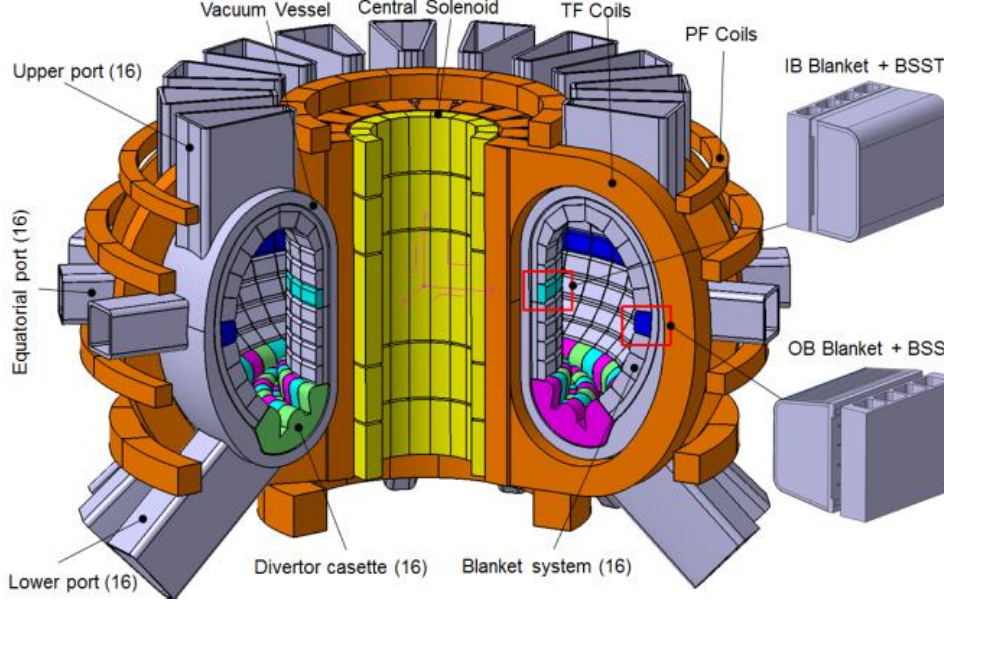
\includegraphics[width=\singleimagewidth]{figures/demo} 
% 	\caption{An example design of a DEMO reactor with solid breeder blankets shown as inboard (IB) and outboard (OB) blanket components.}
% 	\label{fig:demo}
% \end{figure}


A solid, non-mobile tritium breeding concept was first introduced by Abdou\etal\cite{Abdou1975} in 1975. The solid breeder concept satisfies the requirements of a breeder unit: transmute lithium into tritium, act as shield to other sensitive equipment and personnel, and convert energy into extractable heat for electricity production. Reference solid breeder designs have converged toward helium-cooled pebble beds (HCPB) of lithium ceramics.  The HCPB design incorporates packed beds of ceramic pebbles (spherical particles) that are filled into containment structures of a reduced-activation steel. In a typical solid breeder module, the breeding volume is subdivided into several alternating layers of neutron multiplication material (generally beryllium) and tritium breeding material. The layers are separated by plates with internal channels for coolant. Coolant is typically a high pressure helium, though some designs call for pressurized water, in spite of the dangers of the highly exothermic reaction of lithium with oxygen from water vapor in the case of coolant leak. The coolant, heated as it passes through the tritium breeding module, proceeds into a standard electricity production cycle. After tritium is generated inside the ceramic, the bred hydrogen isotope diffuses through the bulk material until being picked up by a low-pressure, slow moving purge gas (primarily helium) and extracted in a closed loop for fuel. Pebble bed forms of tritium breeding volumes have several advantages which include: ease of assembly of granular materials into complex geometries; bred tritium can be readily removed \textit{via} a helium purge gas through interstitial porous networks; ceramic material is unaffected by the large magnetic fields confining the plasma, and temperature gradients across any single pebble are small enough to avoid damage from thermal stress. A sketch of a generic volume of ceramic pebble bed is given in \Cref{fig:solid-breeder-sketch}

\begin{figure}[ht]
	\centering
	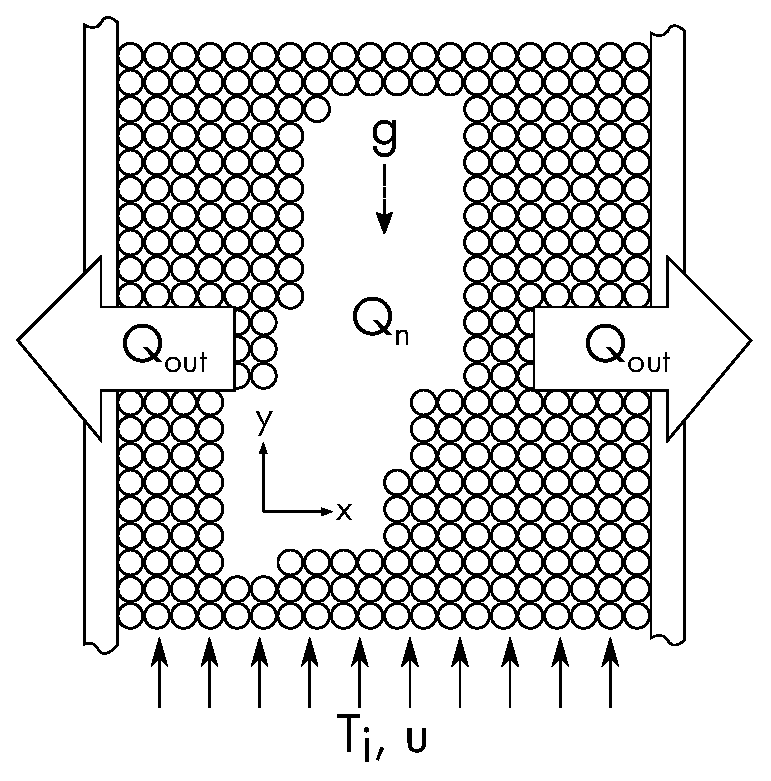
\includegraphics[width=\singleimagewidth]{figures/x-domain.eps} 
	\caption{Sketch of a typical unit of a pebble bed tritium breeding zone. The pebble bed is cooled with contact to the containing structure.}
	\label{fig:solid-breeder-sketch}
\end{figure}

A relatively narrow operational temperature window for optimum breeding performance of ceramics must be observed to respect temperature-dependent phenomena driving tritium release from lithiated ceramic pebbles, as will be discussed in detail in the following section. It is therefore necessary to have accurate knowledge of ceramic pebble bed thermomechanical behavior and comprehensive characterization; reliable models of heat transfer in solid breeders are critical for solid breeder designs. However, temperature prediction in ceramic pebble beds remains a challenge for many reasons. After packing the ceramic pebbles into a containment structure, there exists a coupling between mechanical forces acting upon beds and their heat transport capabilities. In addition, some amount of restructuring of the pebble bed and the internal contact force network is likely to occur in HCPBs from crushing/cracking of individual pebbles, inter-pebble sintering, or creep during operation. Contact conduction in beds, intimately linked to the packing structure, will subsequently be impacted during operation of ceramic pebble beds in fusion reactors. Concurrently, interaction of the slow-moving purge gas with tightly packed pebble beds is an additional route of heat transfer that must be understood. Thus, heat transfer in pebble beds is quite different from standard solid materials and requires specialized modeling of the synergistic physics. Knowledge and characterization of thermal transport must anticipate changes to the heat transfer capabilities and predict temperature profiles for pebble bed packing structures that will emerge after initially-packed pebble beds react to prolonged exposure to fusion reactor environments.

\section{Solid Breeder Thermal Management and Imposed Temperature Window}

To understand the importance of predictive capabilities of temperature in solid breeders, we first consider that one of the main roles of the breeder is to allow tritium to be readily extracted. Thus we need to understand tritium's journey from generation until it is swept away in helium purge gas. The process is shown schematically in \Cref{fig:mechanisms_tritium_transport}. Tritium begins its life internally inside a pebble's bulk. Tritium then diffuses most-slowly through the ceramic lattice until reaching a grain boundary. Along grain boundaries tritium diffuses more quickly and proceeds until reaching a surface of open porosity where it may desorb into the stagnant gas in a pebble's open porosity. Finally, tritium diffuses more rapidly still through the gas until being swept up in the advection of helium purge gas.\cite{Federici1990} 

\begin{figure}[ht]
    \centering
    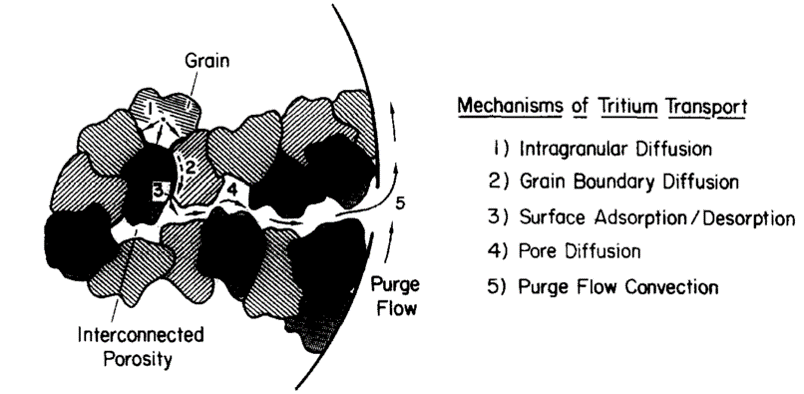
\includegraphics[width=\singleimagewidth]{figures/mechanisms_tritium_transport} 
    \caption{Mechanisms of tritium transport in a single pebble\cite{Federici1990}.}
    \label{fig:mechanisms_tritium_transport}
\end{figure}

Experiments on tritium inventory have attempted to quantify the speeds of tritium release and found that bulk diffusion of tritium, typically the slowest transport mode, is a direct function of temperature.\cite{Franza2013} Thus the lower temperature limit, $T_\text{min}$, of temperature windows for solid breeders, is based on the unacceptable tritium inventory due to slow bulk diffusion. The value of $T_\text{min}$ is generally around \SI{300}{\celsius}. Using the same model of tritium transport, bulk diffusion also limits the maximum temperature in the solid breeder temperature window. At the other end of temperature spectrum, exposure to prolonged high temperature environments causes individual grains in a pebble to grow. Grain growth therefore extends the characteristic length of the slowest mode of tritium transport. Consequently, the maximum temperature, $T_\text{max}$, of the operational window for ceramic pebble beds is generally placed around 80\% of the melt temperature of the ceramic, $T_\text{max} = 0.8 T_\text{melt}$, to avoid surface sintering. For many lithium ceramics, this value falls around \SI{900}{\celsius}.

As a consequence of the tritium release from the solid breeder material, we are faced with a relatively narrow operational temperature to which solid breeder designers must adhere. Thus to provide designers the ability to optimize breeder volumes for tritium breeding and subsequent tritium release, we must understand the important physics and phenomena dictating thermomechanical responses of pebble beds during operation in a fusion reactor.




% High energy (14 MeV) neutrons are ejected from the deuterium-tritium reaction, as described by \Cref{eq:dt-reaction}
% \begin{align}
%     \mathrm{D} + \mathrm{T}&\xrightarrow{}\ ^4\mathrm{He}+\mathrm{n}+17.58\ \text{MeV} \label{eq:dt-reaction}
% \end{align}
% thus t

Tritium breeding blankets will experience high volumetric heating as deposited by high-energy neutrons that are carrying away approximately 80\% of the fusion reaction energy as well as secondary $\gamma$ rays. The deposited heat must be transported through the pebble bed region into the walls of the containing structure, then ultimately into the coolant gas. Heat deposited into pebble beds will transfer \textit{via} inter-particle contact conduction, inter-particle radiation, and convection with the helium purge gas. At the interface with the structural material, similar modes of heat transfer are present: particle-wall contact conduction, particle-wall radiation, and communication \textit{via} helium purge gas convection. As the pebbles heat under the nuclear load, thermal expansion of the pebbles in the packed volume will be contained by cooler structural material. Confined expansion will give rise to increased contact pressure between pebbles. Pressure on pebble beds is known to be the cause of many phenomena, some of which directly impact the thermal transport characteristics of pebble beds and may ultimately jeopardize the reliable and safe operation of breeding blankets. 

The packing structure of packed beds can be considered as a metastable configuration that will last indefinitely unless acted upon by an external perturbation such as vibration or compressive pressure.\cite{Jaeger1996} The ability of a metastable configuration to resist perturbations can in some way be quantified by the initial packing fraction. For more compliant beds, with lower packing fractions, stresses from thermal expansion can cause significant rearrangement of the packing structure which is not recoverable after stress removal. This phenomena has been observed in numerous experiments as so-called plastic rearrangement of pebble beds.\cite{Reimann:2002kl,Reimann:2000tw,Zhang2015} Plasticity of beds may have significant consequences for the ability of the pebble bed to maintain contact with the containing structure and routes for heat out of the bed due to gap formation between pebble volumes and coolant walls. Moreover, increased pressure between pebbles can cause the brittle pebbles themselves to fragment which will also disrupt paths of heat in the inter-particle conduction network. The consequence of both aformentioned effects is an increase in the temperature of bed pebbles. If the fragments are sufficiently small, they may even cause blockage of the helium purge gas. 

Due to the complicated nature of granular materials such as ceramic pebble beds, heat transfer in these solid breeder volumes should not be considered as a static phenomena that can be characterized prior to inserting pebbles beds into breeder modules and then expected to behave consistently after long exposure to fusion environments. Pebble bed temperatures, linked to the packing, will evolve in ways that are currently not predictable and must be studied and modeled.

In spite of their many engineering applications, heat transfer mechanisms in packed beds of granular material are still not thoroughly understood nor characterized. Hence, one approach is to treat the granular material as a fictitious continuous media, an approach adopted by several designers of solid breeders. Many experiments have been carried out for developing phenomenological models for effective material properties. In this approach, heat transport in pebble beds is often characterized with an effective thermal conductivity, $\keff$, and interface heat conductance. Many models have shown their ability to accurately predict the temperature profiles for pebble beds under specific operating conditions. However, the accuracy of the model predictions often degrade as soon as a pebble bed's granular material, grain radii distributions, or operating conditions vary from the experimentally studied packed beds. In addition, propensity for creep, crushing, and inter-particle sintering of ceramic materials alter the packing structure in ways not currently predictable with the effective material characterizations. Furthermore, effective conductivity models that consider interstitial gas often assume the gas is stagnant. The assumption has not been thoroughly vetted and is likely insufficient to capture the thermal influence of the helium purge gas flowing through the ceramic pebble beds in fusion reactors.

To overcome the limitations of effective material modeling, and aided by the acceleration and availability of computational power, many researchers of granular heat transfer have shifted their attention to studies of the interacting physics on pebble-scales. In this approach, we interrogate heat transfer on the scale of contact conductance between interacting particles and directly model transient behaviors of packed beds. We can then couple particle-scale models of heat transfer and mechanics to either volume-averaged fluid models or models of the entire tortuous fluid flow through the porous network of packed beds.


\section{Objectives of this Study}\label{sec:intro-scope-of-work}
% from the intro originally, fit this in with the paragraph below.
The goal of this work is to develop more comprehensive and accurate models for predicting temperature distributions in ceramic breeder pebble beds, accounting for many important phenomena including pebble crushing and fragmentation, dynamic analysis of packing restructuring, and considerations of slow moving inter-porous helium purge gas. The modeling will be done with discrete element method (DEM) models coupled to computational fluid dynamics (CFD) and lattice-Boltzmann (LBM) descriptions of fluid flow. In particular I will study in detail the relationship between topological changes to packing structures, arising from fragmented pebbles, and the resulting changes to heat transfer in packed beds. I will be concerned with the nuclear heating of pebble fragments as they redistribute through pebble beds and come to rest without strong mechanical contact (and therefore contact conductance) to neighboring pebbles. This includes analyzing changes to temperature distributions in pebble beds with different models of pebble damage, analyzing the impact of helium flow on temperatures in beds with fragmented pebbles, and changes to bed stresses and contact forces in beds with restructured packing. Moreover, I will consider changes to effective thermal conductivity in packed beds with simulated irradiation damage induced reduction in solid conductivity of ceramic pebbles. The study will provide blanket researchers with operability margins inside which their designs can tolerate irradiation damage or crushed pebbles.

% In support of the numerical objectives, experimental campaigns of crushing various lithium ceramic pebbles (\lit~and \lis) between two nickel-based steel alloys will be carried out at temperatures ranging from room temperature to \SI{650}{\celsius} to observe the temperature-dependence of crush strength. From the experimental data, I will also validate the Hertzian assumption for contact mechanics of the spherical pebbles on the flat pistons; experiments measure the force-travel response of individual pebbles and, \textit{via} comparison with predictions of Hertz theory, will show a modified Young's modulus is necessary for use in the material inputs. The crush experiments will also be used as a basis for developing a criteria for prediction of pebble crushing in packed beds. 

% Numeric campaigns will develop in stages. In the first stage, many components of the pebble bed modeling will be tested individually. Simulations strictly of heat transfer dependence on pebble interactions (without consideration of fluid flow) will be executed to analyze the links between pebble descriptions (\textit{e.g.} packing fraction, coordination number, contact forces) and temperature distributions in pebble beds with specific models of pebble damage. A study will apply the modified Young's modulus model to show the dependence of crush predictions and external measured stresses of beds on the Young's modulus assigned to pebbles in simulations. Finally, another separate study will assess the impact of fragment size on packing resettling and its role in thermal transport.

% In the second stage, pebble beds similar to the first stage will be analyzed, with and without helium flow. In this stage, the helium flow will be two-way coupled to the pebble bed with fluid phase being characterized with volume-averaged conservation equations. We will see the role of helium on smoothing out temperatures between pebbles which have poor mechanical contact with neighbors in the assembly. Again, effective thermal conductivity measurements will be reported from well-packed beds and beds with pebble damage. Lastly, in this stage, several ITER-relevant configurations of pebble beds are studied. 

% In the third stage, pebble beds are one-way coupled to models of helium flow. Rather than considering volume-averaged conservation equations, we will make use of the novel approach of solving lattice-Boltzmann equation on discretized lattice nodes which allow for simple application of boundary conditions on the complex geometry of packed beds. This approach will provide a more complete view of helium's serpentine route through the pebble bed and its impact on temperature distributions in beds.



%A more thorough understanding of temperature distributions allows for higher confidence in tritium release from pebble beds as well as the potential for increased power density during operation of the solid breeders. 

% One last note: there are other long-term effects expected in the materials experiencing prolonged exposure to cycling irradiation, heat, and stress that have not been discussed here. These loads can lead to thermal ratcheting, irradiation swelling, sintering, or thermally-induced creep which also lead to evolutions in thermophysical properties -- even in the absence of cracked pebbles. These phenomena need to be addressed in time but are, however, beyond the scope of this dissertation. 
% \section{Dissertation Outline}
% In the next chapter I will present a literature review on the state of the art of modeling granular materials and packed beds, including: effective thermal conductivity experiments and their derivative empirical relationships, convective energy exchange in packed bed media, and drag of fluid flow through packed beds. The literature review also discusses the specific application of granular research for packed beds in the fusion community, highlighting progress made and where deficiencies in research remain. In \Cref{ch:modeling-development}, I will present the theory behind the discrete element method modeling for granular interaction as well as experimental efforts to validate Hertz theory and aid in development of pebble damage modeling. Then \Cref{ch:cfd-dem-modeling-development} covers the coupling of the pebble model in DEM to the volume-averaged CFD as well as coupling to solvers of the lattice-Boltzmann equation. After model development is complete, in \Cref{sec:dem-studies}, I begin application of the models to study of temperature distributions in ceramic pebble beds for tritium breeding; first models are run only in the DEM environment, then with the coupled CFD-DEM models, and finally with coupled DEM-LBM simulations. Finally in \Cref{sec:summary} a summary of the work, the impact of the results, and a suggestion for future work will be presented.